\documentclass[a4paper, 12pt]{article}
\usepackage[a4paper,top=1.5cm, bottom=1.5cm, left=1cm, right=1cm]{geometry}
\usepackage{cmap}					% поиск в PDF
\usepackage{mathtext} 				% русские буквы в фомулах
\usepackage[T2A]{fontenc}			% кодировка
\usepackage[utf8]{inputenc}			% кодировка исходного текста
\usepackage[english,russian]{babel}	% локализация и переносы

\usepackage{amsmath}
\usepackage{indentfirst}
\usepackage{longtable}
\usepackage{graphicx}
\usepackage{array}


\title{Работа 1.1.3. Статистическая обработка результатов многократных измерений}
\author{Александр Рожков}
\date{Сентябрь 2023}

\begin{document}

    \maketitle

    \textbf{Цель работы:} применение методов обработки экспериментальных данных при измерении сопротивлений

    \textbf{В работе используются:} набор 270 сопротивлений имеющих номинал 500 Ом, универсальный цифровой мультиметр, работающий в режиме "измерение сопротивлений постоянному току".

    Результаты измерения сопротивлений 270 резисторов (в Омах) приводятся на рис. 1 в порядке возрастания.

    Рассчитаем интервалы измерения сопротивлений для $m = 10$ и $m = 20$

    \begin{equation*}
        \Delta R = \frac{R_{макс} - R_{мин}}{m}
    \end{equation*}

    \begin{equation*}
        \Delta R_{10} = \frac{R_{макс} - R_{мин}}{m} = \frac{505.3\ Ом - 497.0\ Ом}{10} = 0.83\ Ом
    \end{equation*}

    \begin{equation*}
        \Delta R_{20} = \frac{R_{макс} - R_{мин}}{m} = \frac{505.3\ Ом - 497.0\ Ом}{20} = 0.415\ Ом
    \end{equation*}

    Результаты на рис. 1 и рис. 2 разделены на цветовые группы по $\Delta R_{10}$ и $\Delta R_{20}$ соответственно.

    \begin{figure}
        \begin{minipage}{0.48\textwidth}
        \centering
         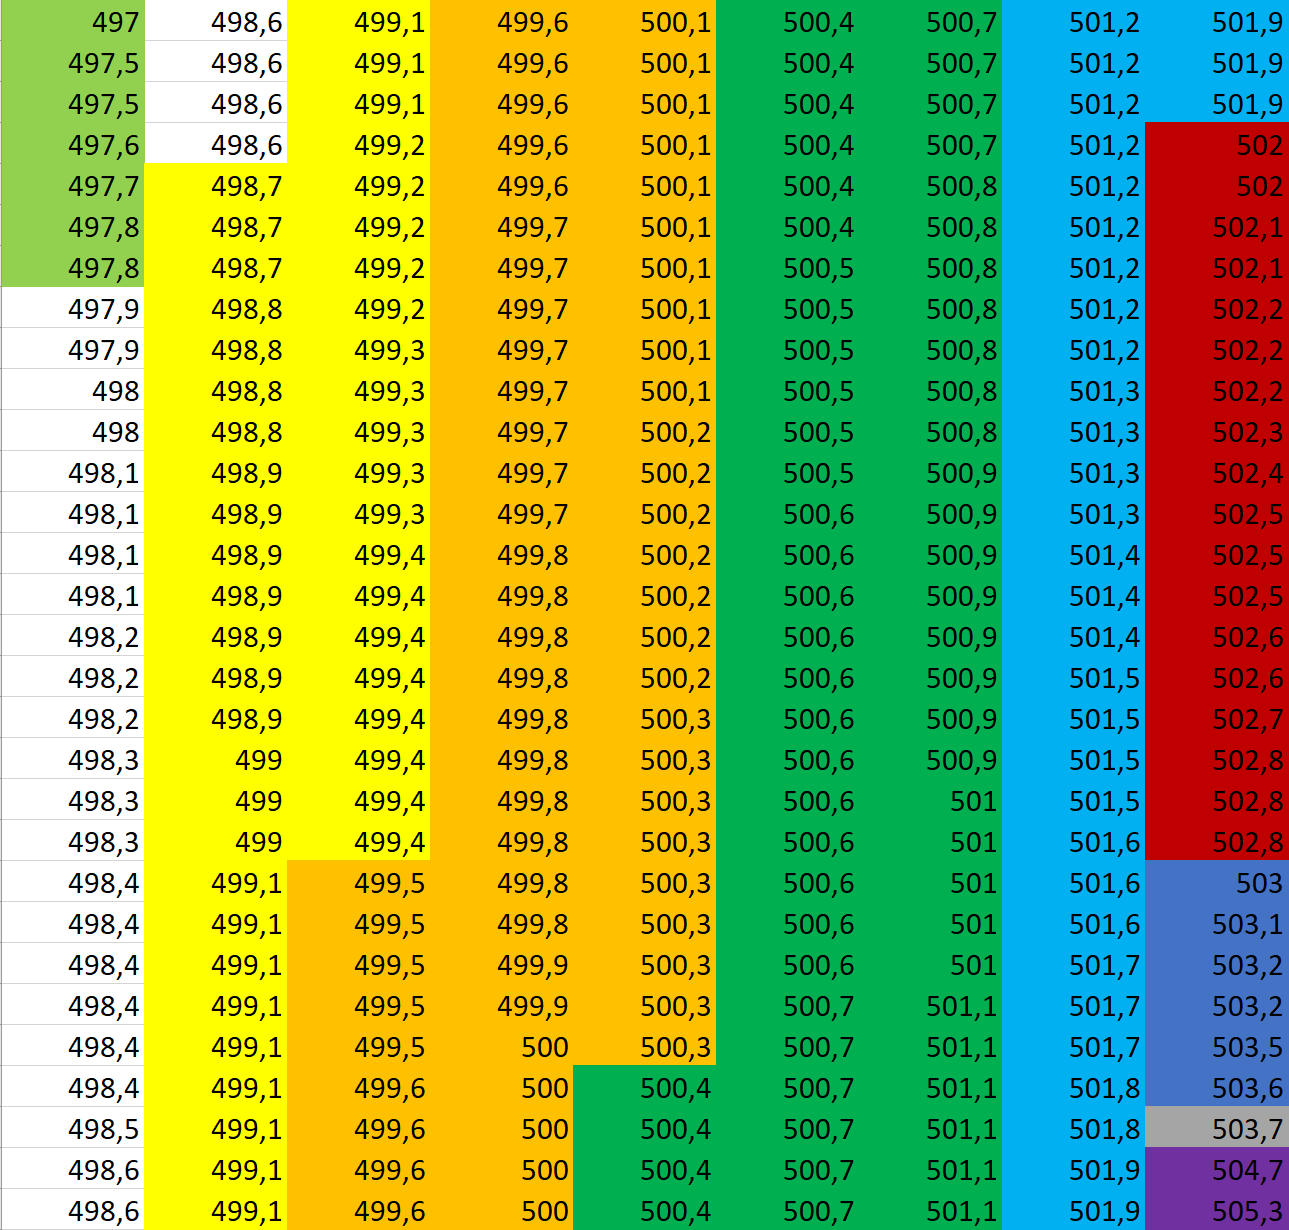
\includegraphics[width=1\linewidth]{Table m10.png}
        \caption{Таблица результатов с цветовым разделением по интервалам измерения при $m = 10$}
        \end{minipage}\hfill
        \begin{minipage}{0.48\textwidth}
        \centering
        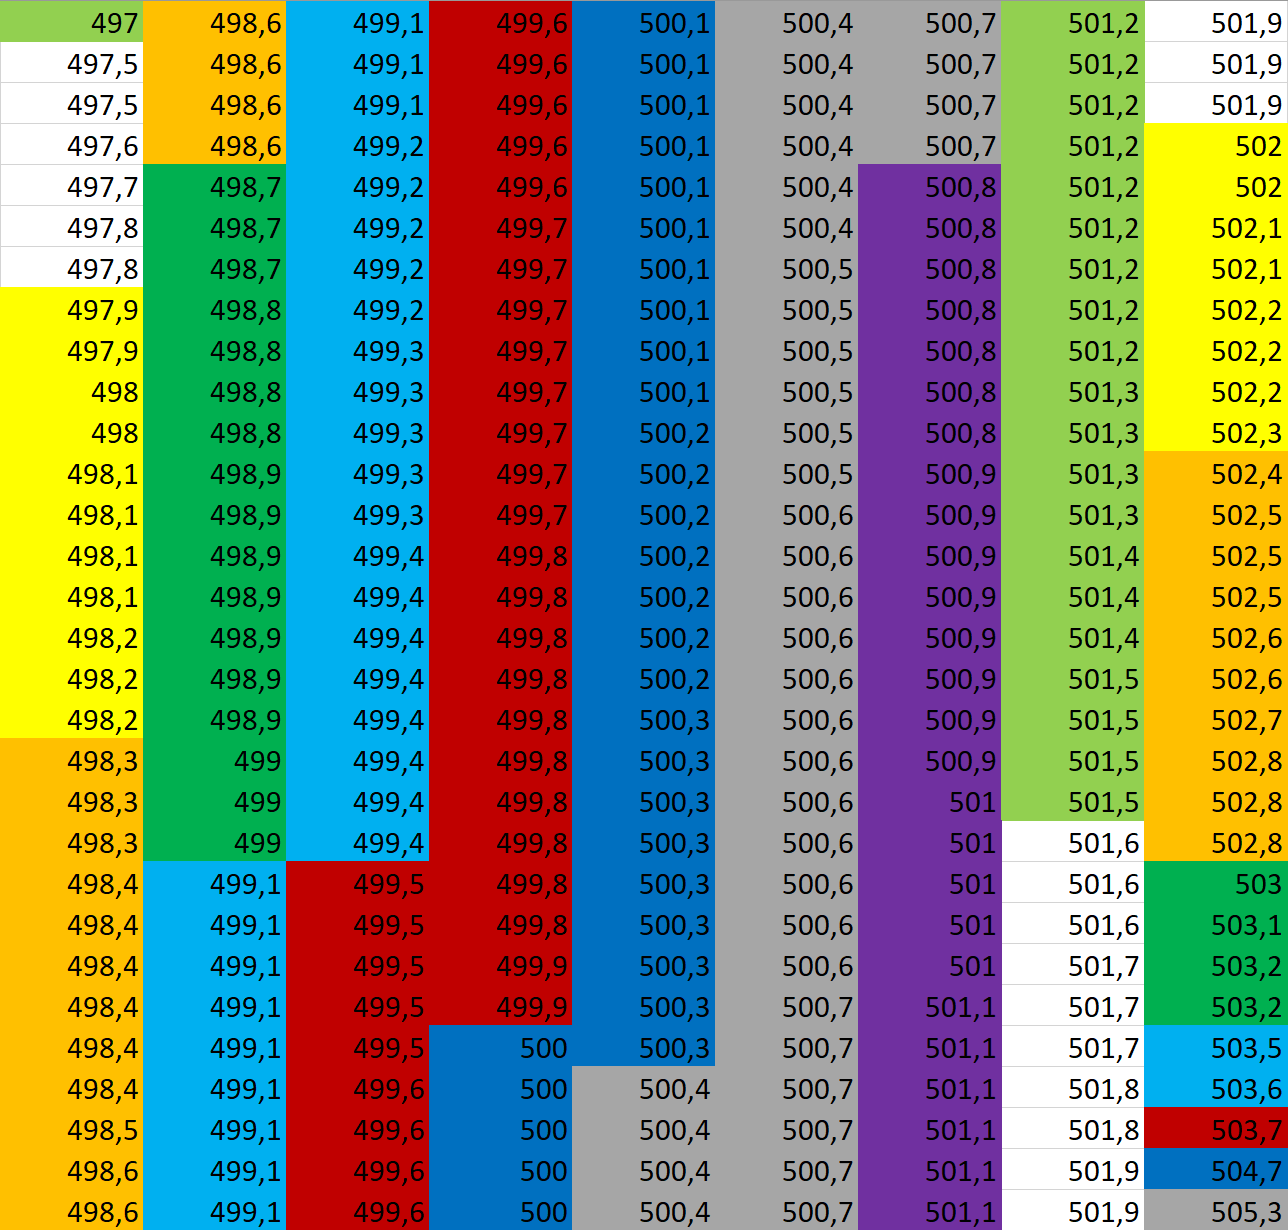
\includegraphics[width=1\linewidth]{Table m20.png}
        \caption{Таблица результатов с цветовым разделением по интервалам измерения при $m = 20$}
        \end{minipage}
    \end{figure}

    По таблице строим гистограммы для $m = 10$ и $m = 20$. Для удобства сравнения с нормальным распределением по оси ординат будем откладывать не число результатов $\Delta n$, попадающих в каждый интервал, а это число, делённое на полное число результатов $N$ и величину интервала $\Delta R$. В таблицах 1 и 2 в зависимости от номера группы $k$ приведены значения $\Delta n$ и $\omega = \Delta n / (N \Delta R)$. На рис. 3 и 4 представлены гистограммы, построенные при помощи библиотеки \textit{matplotlib} языка \textit{python}. Среднее значение сопротивлений находим по формуле:

    \begin{equation}
        \langle R \rangle = \frac{1}{N} \sum_{i=1}^{N} R_i = 500.2\ Ом
    \end{equation}

    Среднеквадратичное отклонение находим по формуле:

    \begin{equation}
        \sigma = \sqrt{\frac{1}{N} \sum_{i=1}^{N}(R_i - \langle R \rangle)^2} = \sqrt{\frac{1}{270}\ 497.9682963} \approx 1.4\ Ом
    \end{equation}

    Расчёты производились при помощи программы \textit{Microsoft Excel}.

    Итого:

    \begin{equation*}
        R = (500.2 \pm 1.4)\ Ом
    \end{equation*}

    \begin{table}[!htbp]
        \centering
        \caption{интервалы изменения для $m = 10$}
        \begin{tabular}{|c|m{1.5em}|m{1.5em}|m{1.5em}|m{1.5em}|m{1.5em}|m{1.5em}|m{1.5em}|m{1.5em}|m{1.5em}|m{1.5em}|}
            \hline
            $k$ & 1 & 2 & 3 & 4 & 5 & 6 & 7 & 8 & 9 & 10 \\
            \hline
            $\Delta n$ & 7 & 27 & 47 & 65 & 64 & 33 & 18 & 6 & 1 & 2 \\
            \hline
            $\omega * 1000$ & 31 & 120 & 210 & 290 & 286 & 147 & 80 & 27 & 4 & 9 \\
            \hline
        \end{tabular}
    \end{table}

    \begin{table}[!htbp]
        \centering
        \caption{интервалы изменения для $m = 20$}
        \begin{tabular}{|c|m{1.5em}|m{1.5em}|m{1.5em}|m{1.5em}|m{1.5em}|m{1.5em}|m{1.5em}|m{1.5em}|m{1.5em}|m{1.5em}|}
            \hline
            $k$ & 1 & 2 & 3 & 4 & 5 & 6 & 7 & 8 & 9 & 10 \\
            \hline
            $\Delta n$ & 1 & 6 & 11 & 16 & 17 & 30 & 34 & 31 & 38 & 26\\
            \hline
            $\omega * 1000$ & 9 & 54 & 98 & 143 & 152 & 268 & 303 & 277 & 339 & 232 \\
            \hline
        \end{tabular}
        \begin{tabular}{|c|m{1.5em}|m{1.5em}|m{1.5em}|m{1.5em}|m{1.5em}|m{1.5em}|m{1.5em}|m{1.5em}|m{1.5em}|m{1.5em}|}
            \hline
            $k$ & 11 & 12 & 13 & 14 & 15 & 16 & 17 & 18 & 19 & 20 \\
            \hline
            $\Delta n$ & 20 & 13 & 8 & 10 & 4 & 2 & 1 & 0 & 1 & 1  \\
            \hline
            $\omega * 1000$ & 178 & 116 & 71 & 89 & 36 & 18 & 9 & 0 & 9 & 9 \\
            \hline
        \end{tabular}
    \end{table}

    \begin{figure}
        \centering
        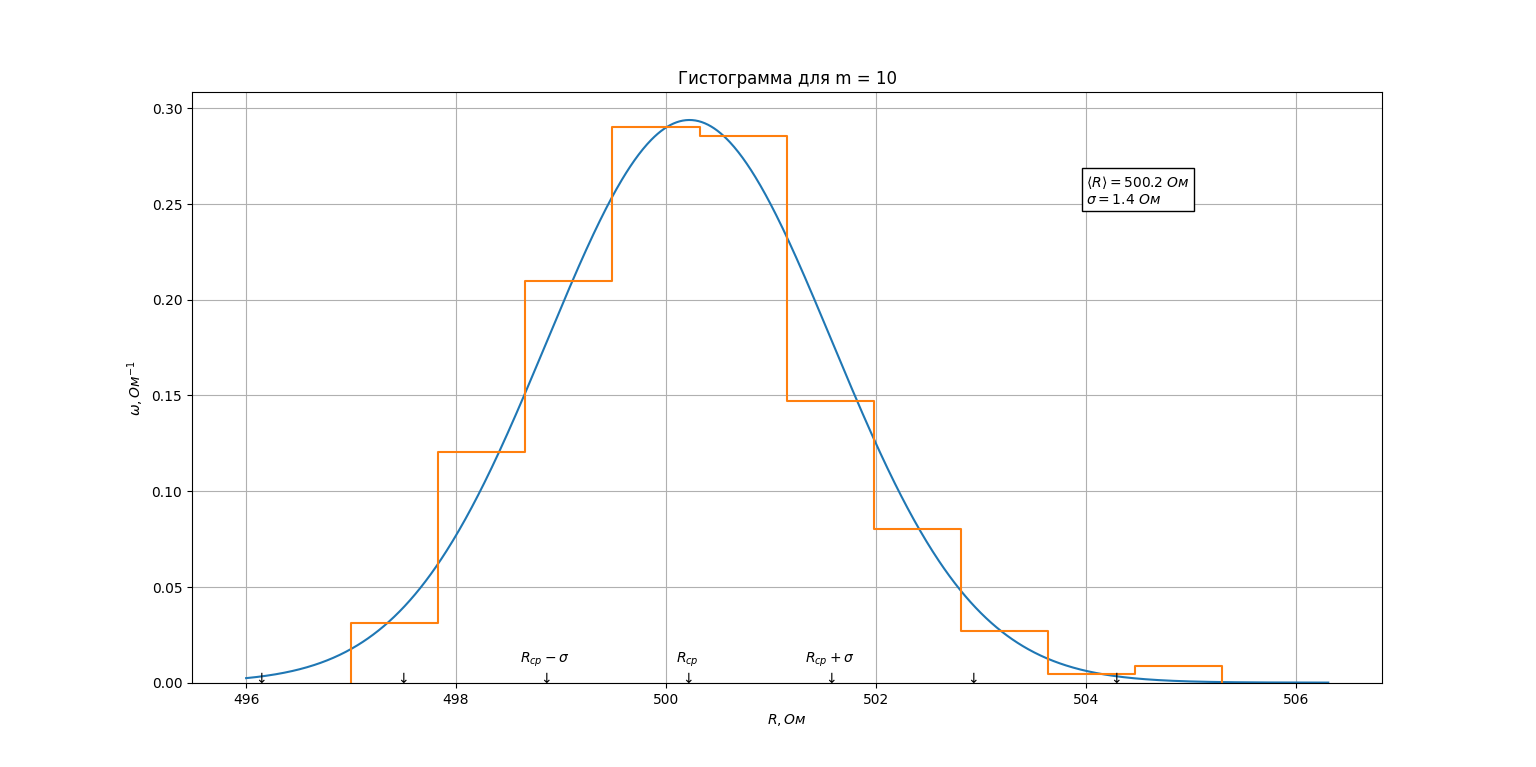
\includegraphics[width=1\linewidth]{m10.png}
        \caption{Таблица результатов с цветовым разделением по интервалам измерения при $m = 10$}
    \end{figure}
    \begin{figure}
        \centering
        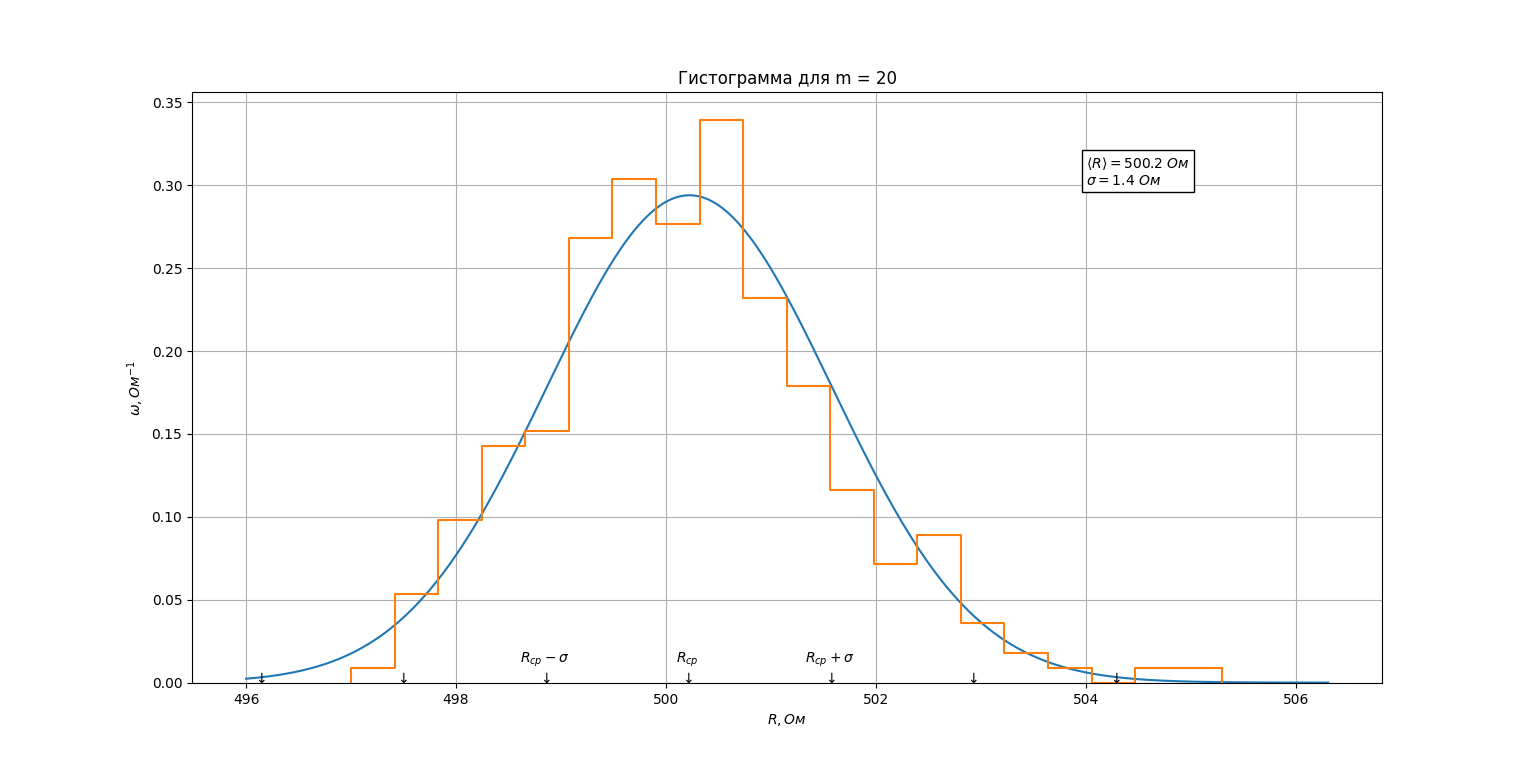
\includegraphics[width=1\linewidth]{m20.png}
        \caption{Таблица результатов с цветовым разделением по интервалам измерения при $m = 20$}
    \end{figure}

    В интервал от $\langle R \rangle - \sigma$ до $\langle R \rangle + \sigma$ попадает 73\% результатов, а в интервал от $\langle R \rangle - 2\sigma$ до $\langle R \rangle + 2\sigma$ соответственно - 97\%. Нормальное распределение описывается формулой:

    \begin{equation}
        y = \frac{1}{\sqrt{2 \pi} \sigma} \exp^{- \frac{(R - \langle R \rangle)^2}{2 \sigma^2}}
    \end{equation}

    Эта функция также изображена на рис. 3 и 4. Видно, что гистограмма соответствует этой зависимости. Теоретическая вероятность попадания измерений в интервал от $\langle R \rangle - \sigma$ до $\langle R \rangle + \sigma$ равна 68\%, а в интервал от $\langle R \rangle - 2\sigma$ до $\langle R \rangle + 2\sigma$ соответственно - 95\%.

    Практически мы получаем, что величина сопротивления резистора, наугад выбранного из данного набора, попадает в интервал $500.2 \pm 1.4\ Ом$ с вероятностью 73\%, в интервал $500.2 \pm 2.8\ Ом$ - с вероятностью 97\%, в интервал  $500.2 \pm 4.2\ Ом$ - с вероятностью 99\%.


\end{document}
